\chapter{Implementacja}
% Temporarily change the margins for this page
\newgeometry{
  left=0.5in,
  right=0.5in,
  top=1.5in,
  bottom=1in,
}
\section{Elementy tworzonego systemu}
\begin{figure}[!htbp]
    \centering
    \includesvg[width=\textwidth]{schemas/master-Dev.drawio.svg}
    \caption{Schemat tworzonego systemu}
    \label{fig:enter-label}
\end{figure}

% Restore the original margins
\restoregeometry
\newpage

\begin{figure}[h!]
    \centering
    \begin{msc}[
        title position=center,
        msc keyword=,
        draw frame=none,
        instance distance=2.5cm,
        left environment distance=0.5cm,
        right environment distance=0.5cm,
        label distance=0.3cm,
        title distance=0.5cm
        ]{Protocol Worker Resource Reservation}
            \declinst{user}{}{User}
            \declinst{protocolWorker}{}{Protocol Worker}
            \declinst{serviceDiscovery}{}{Service Discovery}
            \declinst{producer}{}{Producer}
            
            \footnotesize
            \nextlevel
            \mess{Request Resource Reservation}{user}{protocolWorker}
            \nextlevel
            \nextlevel
            \mess{Query All Registered Producers}{protocolWorker}{serviceDiscovery}
            \nextlevel
            \nextlevel
            \nextlevel
            \mess{List of Producers}{serviceDiscovery}{protocolWorker}
            \nextlevel
            \nextlevel
            \nextlevel
            \inlinestart{loop1}{loop for each Producer}{protocolWorker}{producer}
            \nextlevel
            \nextlevel
            \nextlevel
            \nextlevel
            \mess{Check Resource Availability}{protocolWorker}{producer}
            \nextlevel
            \nextlevel
            \nextlevel
            \mess{Resource Availability}{producer}{protocolWorker}
            \nextlevel
            \nextlevel
            \inlineend{loop1}
            \nextlevel
            \nextlevel
            \mess{\parbox{3cm}{Processing producers for products}}{protocolWorker}{protocolWorker}
            \nextlevel
            \nextlevel
            \nextlevel
            \nextlevel
            \nextlevel
            \mess{Return Resource Availability}{protocolWorker}{user}
        \end{msc}
    \caption{ Schemat wymiany wiadomości podczas przetwarzania żądania użytkownika}
    \label{fig:enter-label}
\end{figure}

\subsection{Rejestr usług}

Głównym elementem w podsystemie użytkowym jest rejestr usług, rejestr ten jest wykorzystywany jako zbiór informacji na temat usług uruchomionych w systemie. W usłudze następuje rejestracja producentów świadczący usługi w systemie oraz węzłów protokołu użytkowników, które są wykorzystywane do zarządzania przydziałem zasobów.

\begin{figure}[!htbp]
    \centering
    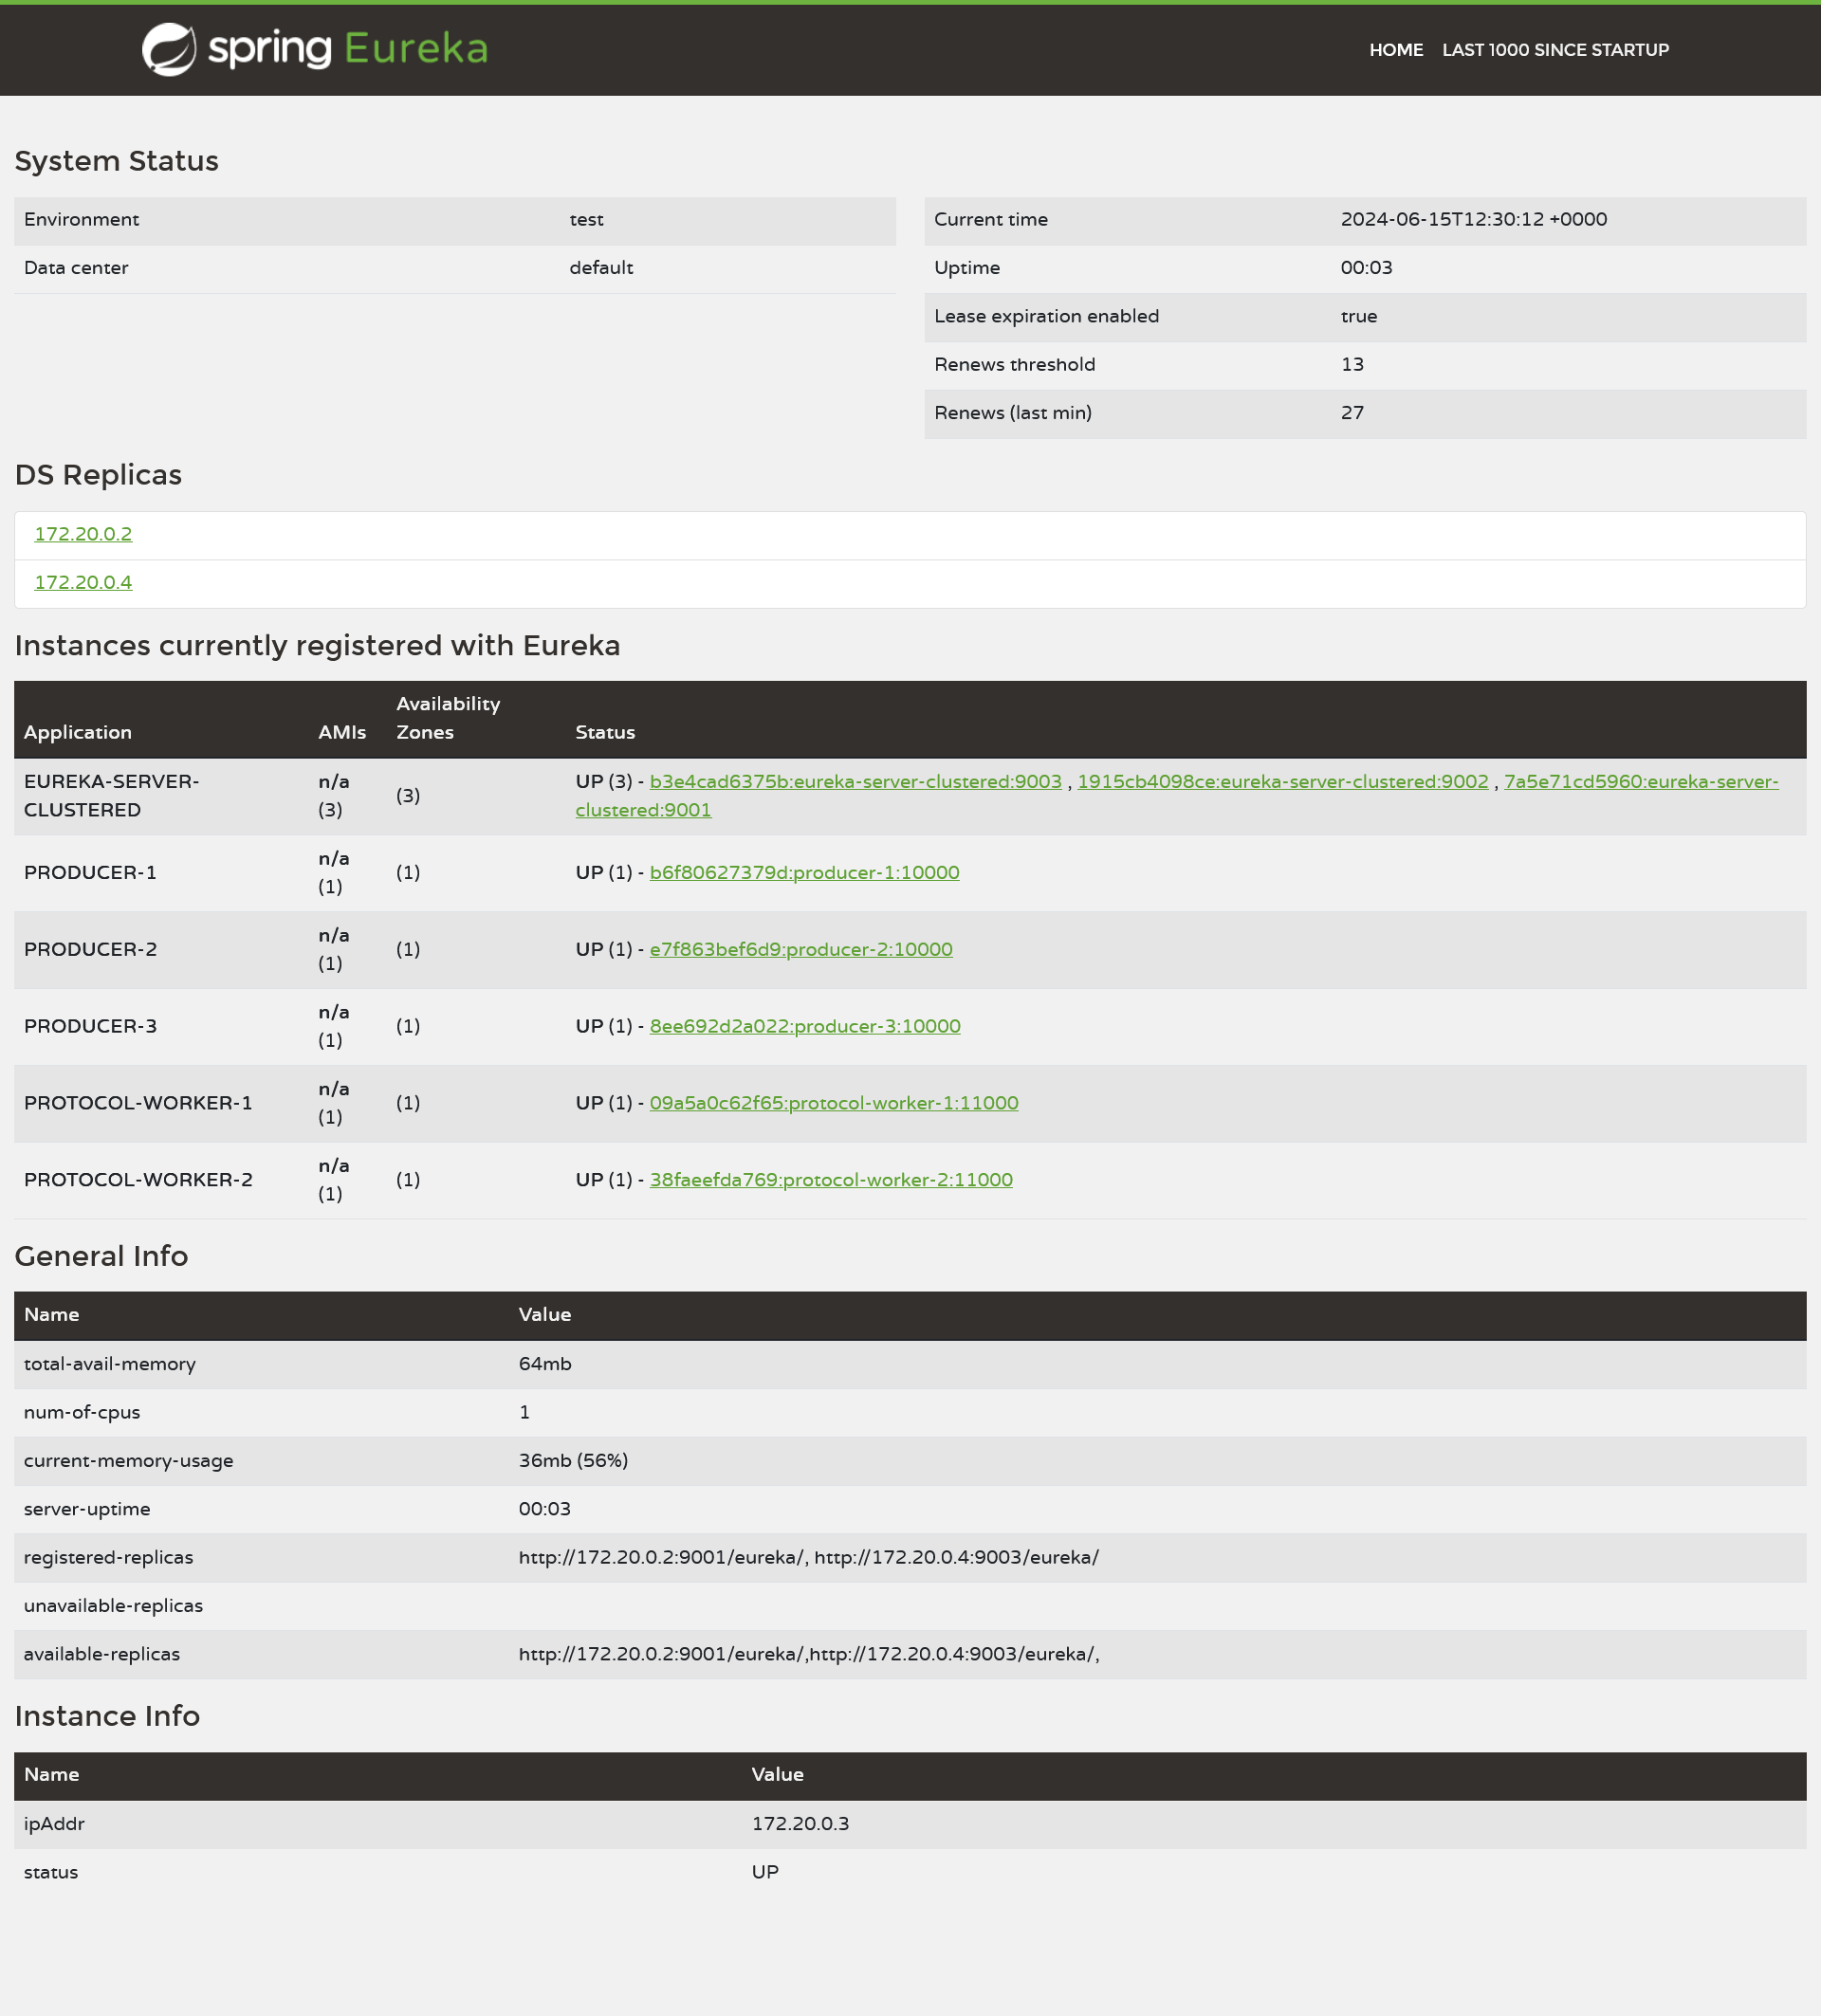
\includegraphics[width=\textwidth]{images/implementation/ServerDiscovery3Producer2Workers.png}
    \caption{Rejestr usług Eureka}
    \label{eurekaServerItems}
\end{figure}

Każda uruchomiona usługa typu producenta oraz węzła protokołu w podsystemie użytkowym jest rejestrowana w usłudze Eureka, gdzie aplikacja przechowywana jest pod unikatową nazwą, która jest wykorzystywana do odpytywania rejestru w usłudze klienckiej w celu otrzymania informacji o działających usługach w systemie. Rejestr przechowuje adresu pod którym usługa jest uruchomiona oraz jej stan. Na rys.\ref{eurekaServerItems} jest przedstawiony przykładowy stan usług zarejestrowanych w rejestrze Eureka.



\begin{lstlisting}[language=Java, caption=Implementacja rejestru usług serwera Eureka]
    
    package com.example.serviceregistry;
    
    import org.springframework.boot.SpringApplication;
    import org.springframework.boot.autoconfigure.SpringBootApplication;
    import org.springframework.cloud.netflix.eureka.server.EnableEurekaServer;
    
    
    @SpringBootApplication
    @EnableEurekaServer
    public class ServiceRegistryApplication {
    
    	public static void main(String[] args) {
    		SpringApplication.run(ServiceRegistryApplication.class, args);
    	}
    }
\end{lstlisting}

Kod usługi rejestru składa się z jednej klasy \verb|ServiceRegistryApplication| oraz metody \verb|main| uruchamiającej aplikacje. Jedyną linijką odróżniającą tę klasę od czystej aplikacji napisanej w frameworku Spring Boot jest adnotacja \verb|@EnableEurekaServer| odpowiada ona za uruchomienie usługi Eureka.

Głównym elementem określającym działanie usługi jest profil Spring Boot oraz wartości przypisane temu profiowi w pliku \verb|application.yml|. 

\subsubsection{Konfiguracja węzła rejestru}

Plik konfiguracyjny \verb|application.yml| jest plikiem YAML podzielony na trzy sekcje, każda opisująca oddzielny profil aplikacji oraz  pola konfiguracyjne niezbędne do prawidłowego działania klastra węzłów rejestru Eureka. 

\begin{lstlisting}[caption=Konfiguracja pierwszego węzła rejestru]
    spring:
      config:
        activate:
          on-profile: peer-1
      application:
        name: eureka-server-clustered
    server:
      port: 9001
    eureka:
      instance:
        preferIpAddress: true
        leaseRenewalIntervalInSeconds: 10
        leaseExpirationDurationInSeconds: 30
      client:
        registerWithEureka: true
        fetchRegistry: true
        serviceUrl:
          defaultZone: ${PEER_2_URL:http://localhost:9002/eureka/},${PEER_3_URL:http://localhost:9003/eureka/}
      server:
        enableSelfPreservation: true
        evictionIntervalTimerInMs: 1000
    logging:
      logstash:
        destinationOne: ${LOGSTASH_DESTINATION_ONE:localhost:5000}
        destinationTwo: ${LOGSTASH_DESTINATION_TWO:localhost:5001}
        destinationThree: ${LOGSTASH_DESTINATION_THREE:localhost:5002}
    
\end{lstlisting}

\subsubsection{Konfiguracja aplikacji}

Pole \verb|spring.config.activate.on-profile| określa, który profil aplikacyjny będzie aktywny podczas inicjalizacji usługi.

Pole \verb|spring.application.name| ustawia nazwę aplikacji na eureka-server-clustered. Nazwa ta jest wykorzystywana do identyfikacji oraz rejestracji aplikacji w klastrze Eureka.

Pole \verb|server.port| określa port urządzenia na którym aplikacja ma być uruchomiona.

\subsubsection{Konfiguracja instancji Eureka}

Pole \verb|eureka.instance.preferIpAddress| wartość tego pola ustawiona na \verb|true| określa preferowanie przez Eureka adresu \akronim{IP} (\english{Internet Protocol}) zamiast nazwy urządzenia do rejestrowania usług.

Pole \verb|eureka.instance.leaseRenewalIntervalInSeconds| ustawia interwał(w sekundach), co który instancja będzie wysyłać informacje o chęci odnowienia dzierżawy.

Pole \verb|eureka.instance.leaseExpirationDurationInSeconds| określa czas trwania(w sekundach), po którym instancja usługi zostanie uznana za wyłączoną, jeżeli aplikacja nie odnowi dzierżawy.

\subsubsection{Konfiguracja klienta Eureka}

Pole \verb|eureka.client.registerWithEureka| wskazuje, że instancja powinna zarejestrować się w serwerze Eureka.

Pole \verb|eureka.client.fetchRegistry| określa, czy ta instancja powinna pobrać informację z rejestru Eureka.

Pole \verb|eureka.client.serviceUrl.defaultZone| określa adresy \akronim{URL} (\english{Uniform Resource Locator}) usług równorzędnych serwerów Eureka w klastrze.

\subsubsection{Konfiguracja serwera Eureka}

Pole \verb|eureka.server.enableSelfPreservation| określa tryb samozachowawczy, który pomaga w utrzymaniu dostępności serwera Eureka nawet w przypadku partycji sieciowej lub dużych opóźnień.

Pole \verb|eureka.server.evictionIntervalTimerInMs| ustawia interwał (w milisekundach), dla którego ma być uruchamiane zadanie usuwania aplikacji których czas dzierżawy wygasł.


plik \verb|application.yml| definiuje ustawienia konfiguracyjne dla aplikacji Spring Boot z różnymi profilami: peer-1, peer-2 i peer-3. Każdy profil konfiguruje aplikację jako część klastrowej konfiguracji serwera Eureka oraz wykorzystuje pozostałe uruchomione serwery Eureka jako repliki swojego rejestru w celu zapewnienia wysokiej dostępności w przypadku awarii jednego z węzłów w klastrze.

\subsection{Producent}

\subsection{Węzeł protokołu}
\subsubsection{Podsystem monitoringu producentów}
\subsubsection{Podsystem propozycji zasobów}

\section{Uruchomienie środowiska}